\chapter{Management Summary}
\section{Ausgangslage}
Die Bedrohung von Industriespionage und Hackerangriffen durch Geheimdienste und organisierte Hackergruppen ist in den letzten Jahren gestiegen, da die Welt immer weiter vernetzt wird und so mehr Möglichkeiten für solche Angriffe bestehen. Gezielte Angriffe mit klaren Motivationen, wie die Industriespionage, setzen auf sogenannte \gls{apt} Attacken. Bei solchen Angriffen kann es Monate bis Jahre dauern, bis der Angreifer Zugriff auf das System erlangt. Der Sinn solch langwieriger Prozeduren ist die Verschleierung des Angriffs. Durch das sehr langsame Kompromittieren des Opfers ist die Wahrscheinlichkeit geringer, entdeckt zu werden. Bei der RUAG und dem Eidgenössischen Departement für auswärtige Angelegenheiten (EDA) wurde eine \gls{apt} Attacke erst nach circa 14 Monaten erkannt, das zeigt wie schwierig es ist, solche Attacken zu erkennen. Wenn so eine Attacke aufgedeckt wird, fallen komplexe Analysearbeiten an, währenddessen schreitet der Angriff weiter fort. Es besteht somit Bedarf, die weitere Kompromittierung des Systems zu verhindern oder zumindest zu verzögern.

\section{Vorgehen}
Die Phase, bei dem das System unterwandert wird, um später Informationen zu exfiltrieren, läuft relativ simpel ab. Eine Software (Malware), die in eine Organisation eingeschleust wurde, sendet in zeitlich grossen Abständen (z.B. 90 Tage) Informationen über den Sicherheitszustand der Organisation an einen sogenannten \gls{cc} Server. Dieser \gls{cc} Server entscheidet, ob die Organisation mit dem aktuellen Sicherheitszustand weiter kompromittiert werden kann. Falls dem so ist, antwortet der \gls{cc} Server mit Befehlen, die die Malware ausführt.\\

Das Ziel der Arbeit besteht darin, Zugriffe auf einen \gls{cc} Server zu erkennen und diese auf einen Fake \gls{cc} Server umzuleiten. Der Fake \gls{cc} Server kann den \gls{cc} Server des Angreifers sowie die Malware so täuschen, dass der Angreifer im Glauben gelassen wird, die Malware funktioniere noch. In Wirklichkeit wird aber keiner der Befehle des \gls{cc} Servers der Angreifer ausgeführt, da diese Befehle aus den Antworten des \gls{cc} Servers herausgefiltert werden.

\section{Ergebnisse}
Aus der Entwicklung von zwei Prototypen entstand die Fish Tank Suite. Sie erhielt ihren Namen durch die verschiedenen Systemelemente, denen Namen von Fischen zugeteilt wurden. Die Fish Tank Suite zeichnet den HTTP/HTTPS Verkehr auf und speichert ihn in eine Datenbank. Die gewonnenen Daten können mit weiteren Informationen angereichert werden. Es wird zum Beispiel nach verschlüsselten Datenpaketen gesucht, die dann entschlüsselt werden. Die Informationen (Schlüssel) um die Datenpakete zu entschlüsselt müssen vorher durch ein Team aus Spezialisten durch eine Analyse des Angriffs erarbeitet werden. Die angereicherten Daten helfen dabei, Zugriffe auf \gls{cc} Server zu erkennen und umzuleiten. Für die Erkennung der \gls{cc} Zugriffe wurden Suchstrategien entwickelt, die auf spezifische Eigenschaften solcher \gls{cc} Zugriffe zielen.  Diese Suchstrategien durchsuchen die Datenbank und setzen eine Umleitung anhand der Zieladresse des \gls{cc} Servers der Angreifer.

\begin{figure}[H]
	\centering
	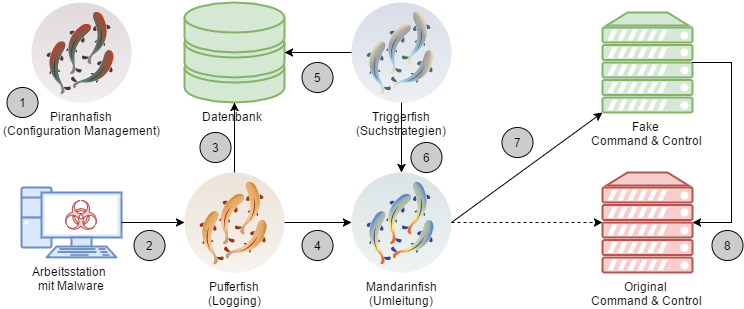
\includegraphics[width=\textwidth]{img/MS-FTS.png}
	\caption{Management Summary: Ergebnis Fish Tank Suite}
	\label{fig:ergebnis_fish_tank_suite}
\end{figure}

\begin{enumerate}
	\item Über den Piranhafish werden alle Instanzen konfiguriert, so dass die Malware erkannt und umgeleitet werden kann.
	\item Die Malware möchte dem Original \gls{cc} Server Informationen über den Sicherheitszustand der Arbeitsstation, auf der er installiert ist, senden. Alle Datenpakete, die ins Internet gehen, müssen aber am Pufferfish vorbei.
	\item Der Pufferfish speichert die Anfrage der Malware in einer Datenbank. In der Datenbank wird bei Bedarf der Inhalt des Datenpakets entschlüsselt.
	\item Die Anfrage der Malware wird aber trotzdem weitergesendet, da noch nicht klar ist, ob es sich um ein ganz normales Datenpaket handelt.
	\item Der Triggerfish durchsucht die Datenbank mit vordefinierten Suchstrategien.
	\item Wenn der Triggerfish das Datenpaket der Malware erkannt hat, teilt er dem Mandarinfish mit, dass er die Verbindung der Malware umleiten soll.
	\item Die Verbindung der Malware wird vom ursprünglichen Ziel, dem Original \gls{cc} Server, auf den Fake \gls{cc} Server umgeleitet.
	\item Der Fake \gls{cc} Server leitet das Datenpaket der Malware an den Original \gls{cc} Server weiter, damit kein Verdacht geschöpft werden kann. Die Antwort des Original \gls{cc} Server kann vom Fake \gls{cc} Server so verändert werden, dass die Malware weiterschläft und somit keine gefährlichen Aktionen mehr durchführt.
\end{enumerate}

Die Fish Tank Suite ist in der Lage eine Malware zu erkennen, umzuleiten und den Originalen \gls{cc} zu täuschen, somit ist der Bedarf, den weiteren Kompromittierungsprozess zu verhindern, erfüllt.

\section{Ausblick}
Die Entwicklung der Fish Tank Suite befindet sich in einem frühen Stadium. Diverse Anforderungen gehörten nicht zum Anforderungskatalog, die in einem realen Softwareprojekt dazu gehören. Trotzdem läuft das System stabil und eignet sich für eine Weiterentwicklung sehr. Die Suchstrategien könnten auch über ein öffentliches Repository ausgetauscht werden, so dass auch andere Organisationen, die mit denselben Problemen konfrontiert sind, davon profitieren können. Darüber hinaus wären auch präventive Installationen solcher Suchstrategien denkbar.